% Compile: pdfLaTeX or LuaLaTeX (Overleaf OK).
% Audience: greenhorns --- what ANN/CAGRA is, and what "filtering" means.
\documentclass[aspectratio=169,11pt]{beamer}

\usetheme{Madrid}
\usecolortheme{whale}
\setbeamertemplate{navigation symbols}{}
\setbeamertemplate{footline}[frame number]
\setbeamerfont{title}{size=\Large\bfseries}
\setbeamerfont{frametitle}{size=\large\bfseries}

\usepackage{booktabs}
\usepackage{tikz}
\usepackage{hyperref}
\usetikzlibrary{arrows.meta,positioning,shapes.geometric,fit,calc}

\title{CAGRA and Filtering --- 101}
\subtitle{Why ``ANN works'' $\neq$ ``filtered ANN works''}
\author{CUDA$\to$HIP / Milvus team}
\date{August 2026}

\begin{document}

%======================================================================
\begin{frame}
  \titlepage
  \vspace{0.4em}
  \begin{center}
    \small
    For colleagues who are not ANN specialists.\\
    Goal: understand \textbf{what filtering is} in vector search,\\
    and why our gfx1100 CAGRA story differs from the AMD Instinct blog.
  \end{center}
\end{frame}

%======================================================================
\begin{frame}{Agenda}
  \begin{enumerate}
    \item What is a vector? What is nearest-neighbor search?
    \item Exact vs Approximate (ANN)
    \item What is CAGRA? (graph index)
    \item Unfiltered search --- what AMD demos
    \item \textbf{Filtering / bitset} --- the missing piece
    \item Why Milvus needs filters
    \item What works / fails on our lab
    \item One-slide takeaway for managers
  \end{enumerate}
\end{frame}

%======================================================================
\section{Vectors}
\begin{frame}{What is a ``vector'' here?}
  \begin{block}{Not a C++ \texttt{std::vector}}
    A list of numbers that represents meaning --- an \textbf{embedding}.
  \end{block}

  \vspace{0.6em}
  \begin{columns}[T]
    \begin{column}{0.55\textwidth}
      \textbf{Example}
      \begin{itemize}
        \item Text: ``What causes tides?''
        \item Model turns it into 128 / 768 / \ldots\ floats
        \item Similar texts $\Rightarrow$ close numbers
      \end{itemize}
    \end{column}
    \begin{column}{0.42\textwidth}
      \centering
      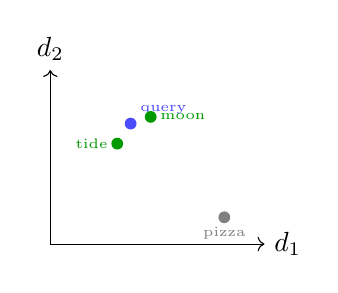
\begin{tikzpicture}[scale=0.85]
        \draw[->] (0,0) -- (3.2,0) node[right] {$d_1$};
        \draw[->] (0,0) -- (0,2.6) node[above] {$d_2$};
        \fill[blue!70] (1.2,1.8) circle (2.5pt) node[above right] {\tiny query};
        \fill[green!60!black] (1.0,1.5) circle (2.5pt) node[left] {\tiny tide};
        \fill[green!60!black] (1.5,1.9) circle (2.5pt) node[right] {\tiny moon};
        \fill[gray] (2.6,0.4) circle (2.5pt) node[below] {\tiny pizza};
      \end{tikzpicture}
    \end{column}
  \end{columns}

  \vspace{0.5em}
  {\footnotesize Database stores millions of such vectors (documents, products, images).}
\end{frame}

%======================================================================
\begin{frame}{The basic question: nearest neighbors}
  \begin{block}{Search}
    Given a \textbf{query vector}, find the $k$ database vectors that are
    \textbf{closest} (smallest distance / largest similarity).
  \end{block}

  \vspace{0.8em}
  \begin{center}
    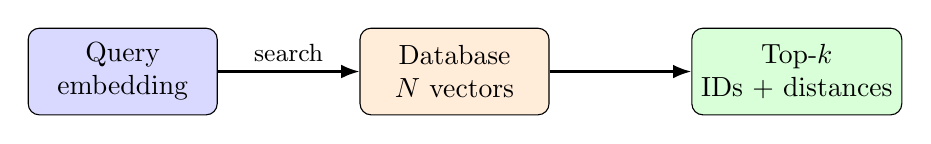
\begin{tikzpicture}[
      box/.style={draw,rounded corners,align=center,minimum height=1.1cm,minimum width=2.4cm},
      arr/.style={-{Latex},thick}
    ]
      \node[box,fill=blue!15] (q) {Query\\embedding};
      \node[box,fill=orange!15,right=1.8cm of q] (db) {Database\\$N$ vectors};
      \node[box,fill=green!15,right=1.8cm of db] (out) {Top-$k$\\IDs + distances};
      \draw[arr] (q) -- (db) node[midway,above] {\small search};
      \draw[arr] (db) -- (out);
    \end{tikzpicture}
  \end{center}

  \vspace{0.8em}
  \textbf{Example:} $k{=}5$ $\Rightarrow$ ``give me the 5 most similar documents.''
\end{frame}

%======================================================================
\section{ANN}
\begin{frame}{Exact search vs Approximate (ANN)}
  \begin{columns}[T]
    \begin{column}{0.48\textwidth}
      \begin{block}{Exact (brute force)}
        Compare query to \textbf{every} vector.\\
        Perfect answers.\\
        Slow when $N$ is huge.
      \end{block}
    \end{column}
    \begin{column}{0.48\textwidth}
      \begin{block}{Approximate (ANN)}
        Use an \textbf{index} to skip most vectors.\\
        Much faster.\\
        May miss a few true neighbors.
      \end{block}
    \end{column}
  \end{columns}

  \vspace{0.8em}
  \textbf{Recall@k} $=$ ``what fraction of the true top-$k$ did we find?''\\
  {\footnotesize 1.0 = perfect; 0.0 = completely wrong / empty results.}

  \vspace{0.6em}
  \textbf{ANN indexes} (examples): IVF-Flat, IVF-PQ, HNSW, \textbf{CAGRA}.
\end{frame}

%======================================================================
\begin{frame}{Why indexes exist (intuition)}
  \begin{center}
    
\begin{tikzpicture}[
      every node/.style={font=\small},
      arr/.style={-{Latex},thick}
    ]
      \node[align=center] (a) at (0,0) {\textbf{No index}\\scan all $N$};
      \node[align=center] (b) at (5.5,0) {\textbf{With index}\\look only near\\promising regions};
      \draw[arr] (a) -- (b) node[midway,above] {build once, search many times};
    \end{tikzpicture}
  \end{center}

  \vspace{1em}
  \begin{itemize}
    \item \textbf{Build} = create the structure (clusters, graph, \ldots)
    \item \textbf{Search} = walk that structure for each query
    \item Trade-off knobs: speed vs recall vs memory
  \end{itemize}
\end{frame}

%======================================================================
\section{CAGRA}
\begin{frame}{What is CAGRA?}
  \begin{block}{One sentence}
    \textbf{CAGRA} = a \textbf{graph}-based ANN index designed for GPUs
    (from NVIDIA cuVS; AMD port = hipVS).
  \end{block}

  \vspace{0.5em}
  \begin{itemize}
    \item Each database vector = a \textbf{node}
    \item Edges connect each node to its nearby neighbors
    \item Search = start somewhere, \textbf{walk the graph} toward the query
  \end{itemize}

  \vspace{0.6em}
  \begin{center}
    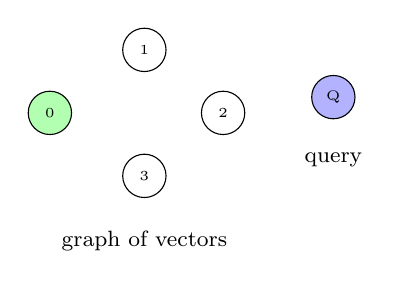
\begin{tikzpicture}[
      n/.style={circle,draw,minimum size=0.55cm,inner sep=0pt,font=\tiny},
      every edge/.style={-{Latex},gray}
    ]
      \node[n,fill=green!30] (0) at (0,0) {0};
      \node[n] (1) at (1.2,0.8) {1};
      \node[n] (2) at (2.2,0) {2};
      \node[n] (3) at (1.2,-0.8) {3};
      \node[n,fill=blue!30] (q) at (3.6,0.2) {Q};
      \draw (0) edge (1) (0) edge (3) (1) edge (2) (3) edge (2) (2) edge (q);
      \node[font=\footnotesize,below=0.3cm of 3] {graph of vectors};
      \node[font=\footnotesize,below=0.3cm of q] {query};
    \end{tikzpicture}
  \end{center}

  \vspace{0.3em}
  {\footnotesize Official Milvus GPU tutorials often lead with \texttt{GPU\_CAGRA}.}
\end{frame}

%======================================================================
\begin{frame}{CAGRA: build vs search}
  \begin{columns}[T]
    \begin{column}{0.48\textwidth}
      \begin{block}{Build}
        \begin{itemize}
          \item Create a knn graph
          \item Optimize / prune it
          \item Store graph (+ often raw vectors)
        \end{itemize}
        {\footnotesize Graph build algo matters:\\
        \texttt{ivf\_pq} vs \texttt{nn\_descent}}
      \end{block}
    \end{column}
    \begin{column}{0.48\textwidth}
      \begin{block}{Search}
        \begin{itemize}
          \item Start from entry points
          \item Expand neighbors on GPU
          \item Keep a candidate heap
          \item Return top-$k$ IDs
        \end{itemize}
        {\footnotesize Knobs: \texttt{itopk\_size}, \ldots}
      \end{block}
    \end{column}
  \end{columns}

  \vspace{0.8em}
  \textbf{``Ordinary build / search''} = search over the \textbf{whole} index.\\
  No extra rule that says ``skip these IDs.''
\end{frame}

%======================================================================
\begin{frame}{What the AMD hipVS blog shows}
  \begin{block}{Blog demo (Instinct)}
    Encode texts $\to$ \texttt{cagra.build(...)} $\to$ \texttt{cagra.search(...)}\\
    Print top passages for a question.
  \end{block}

  \vspace{0.6em}
  That is \textbf{unfiltered} search:
  \begin{itemize}
    \item Every vector in the index is allowed
    \item No ``deleted'' / ``hidden'' / ``not permitted'' set
  \end{itemize}

  \vspace{0.5em}
  \begin{center}
    \large Unfiltered $=$ ``search everything that was indexed.''
  \end{center}
\end{frame}

%======================================================================
\section{Filtering}
\begin{frame}{What is filtering? (plain English)}
  \begin{block}{Filtering}
    During search, some database rows are \textbf{forbidden}.\\
    The engine must return nearest neighbors \textbf{only among allowed} rows.
  \end{block}

  \vspace{0.6em}
  \textbf{Everyday analogies}
  \begin{itemize}
    \item Soft-delete: document removed, but not yet purged from the index
    \item ACL: user may only see vectors from \emph{their} tenant / project
    \item Predicate: ``only products in stock'', ``only English docs''
  \end{itemize}

  \vspace{0.5em}
  Without filtering you would keep returning deleted or forbidden IDs.
\end{frame}

%======================================================================
\begin{frame}{Tiny example (ids 0\ldots7)}
  \footnotesize
  Database has 8 vectors. Query wants top-1.\\[0.4em]

  \begin{center}
  \begin{tabular}{@{}clc@{}}
    \toprule
    ID & Status & Allowed? \\
    \midrule
    0 & deleted & no \\
    1 & ok & \textbf{yes} \\
    2 & ok & \textbf{yes} \\
    3 & deleted & no \\
    4--7 & ok & \textbf{yes} \\
    \bottomrule
  \end{tabular}
  \end{center}

  \vspace{0.6em}
  \begin{itemize}
    \item \textbf{Unfiltered:} nearest might be ID \texttt{0} (deleted) --- bad for the app
    \item \textbf{Filtered:} must pick nearest among \{1,2,4,5,6,7\}
  \end{itemize}

  \vspace{0.4em}
  Same index, same query --- \textbf{different allowed set}.
\end{frame}

%======================================================================
\begin{frame}{How the GPU is told: a bitset}
  \begin{block}{Bitset (bit mask)}
    One bit per database row: allowed or not.
  \end{block}

  \vspace{0.5em}
  \begin{center}
  \texttt{ID:   0 1 2 3 4 5 6 7}\\[0.2em]
  \texttt{mask: 0 1 1 0 1 1 1 1}\\[0.2em]
  {\footnotesize (example polarity: 1 = allowed --- as in cuVS/hipVS Python)}
  \end{center}

  \vspace{0.7em}
  \begin{itemize}
    \item Compact: 1 million vectors $\approx$ 125 KB
    \item Passed into search: ``skip bits that are 0''
    \item In Python hipVS/cuVS: \texttt{filters.from\_bitset(...)}
    \item In Knowhere/Milvus tests: \textbf{BitsetView} (often opposite polarity:\\
          bit set = excluded --- conversions matter)
  \end{itemize}
\end{frame}

%======================================================================
\begin{frame}{Unfiltered vs filtered (picture)}
  \begin{center}
    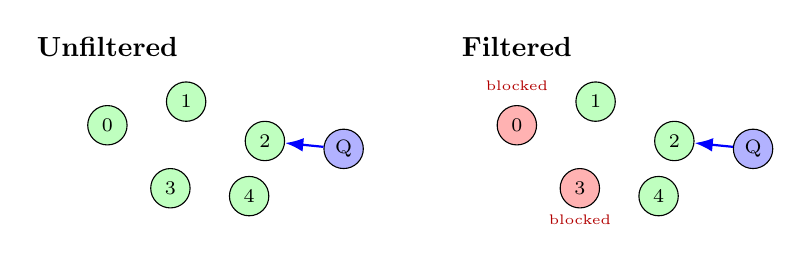
\begin{tikzpicture}[
      n/.style={circle,draw,minimum size=0.5cm,inner sep=0pt,font=\scriptsize},
      arr/.style={-{Latex},thick}
    ]
      % left
      \node[font=\bfseries] at (0,2.2) {Unfiltered};
      \foreach \i/\x/\y in {0/0/1.2,1/1/1.5,2/2/1.0,3/0.8/0.4,4/1.8/0.3} {
        \node[n,fill=green!25] (\i) at (\x,\y) {\i};
      }
      \node[n,fill=blue!30] (q1) at (3.0,0.9) {Q};
      \draw[arr,blue] (q1) -- (2);

      % right
      \begin{scope}[shift={(5.2,0)}]
        \node[font=\bfseries] at (0,2.2) {Filtered};
        \node[n,fill=red!30] (0) at (0,1.2) {0};
        \node[n,fill=green!25] (1) at (1,1.5) {1};
        \node[n,fill=green!25] (2) at (2,1.0) {2};
        \node[n,fill=red!30] (3) at (0.8,0.4) {3};
        \node[n,fill=green!25] (4) at (1.8,0.3) {4};
        \node[n,fill=blue!30] (q2) at (3.0,0.9) {Q};
        \draw[arr,blue] (q2) -- (2);
        \node[font=\tiny,red!70!black] at (0,1.7) {blocked};
        \node[font=\tiny,red!70!black] at (0.8,-0.0) {blocked};
      \end{scope}
    \end{tikzpicture}
  \end{center}

  \vspace{0.4em}
  Red nodes must never appear in the result list.
\end{frame}

%======================================================================
\begin{frame}{Why filtering is harder than it sounds}
  ANN search does \textbf{not} scan all IDs.\\
  It walks a graph / probes clusters.

  \vspace{0.6em}
  With a filter, the algorithm must:
  \begin{enumerate}
    \item Ignore forbidden nodes when expanding candidates
    \item Still find enough \textbf{allowed} neighbors
    \item Keep recall high even if 40\%--98\% of rows are blocked
  \end{enumerate}

  \vspace{0.6em}
  \begin{block}{Failure modes (what we see)}
    \begin{itemize}
      \item Return \textbf{wrong} allowed IDs $\Rightarrow$ recall $\approx 0$
      \item Return \textbf{empty} (\texttt{-1} / ``no neighbor'') $\Rightarrow$ recall $= 0$
    \end{itemize}
  \end{block}
\end{frame}

%======================================================================
\section{Milvus}
\begin{frame}{Where filtering shows up in Milvus}
  \begin{itemize}
    \item \textbf{Delete / TTL:} row gone from the logical collection,\\
          still present in a segment index until compact
    \item \textbf{Scalar predicates:} \texttt{color == "red"} combined with vector search
    \item \textbf{Multi-tenancy / visibility:} hide other users' rows
  \end{itemize}

  \vspace{0.7em}
  Knowhere Catch2 tests this with a \textbf{bitset} on GPU indexes\\
  (\texttt{Search With Bitset}, \texttt{Simple Bitset}).

  \vspace{0.5em}
  {\footnotesize If bitset search is broken, ``plain RAG demo'' may look fine,\\
  while production delete/filter paths are not.}
\end{frame}

%======================================================================
\begin{frame}{Stack: who does what}
  \begin{center}
    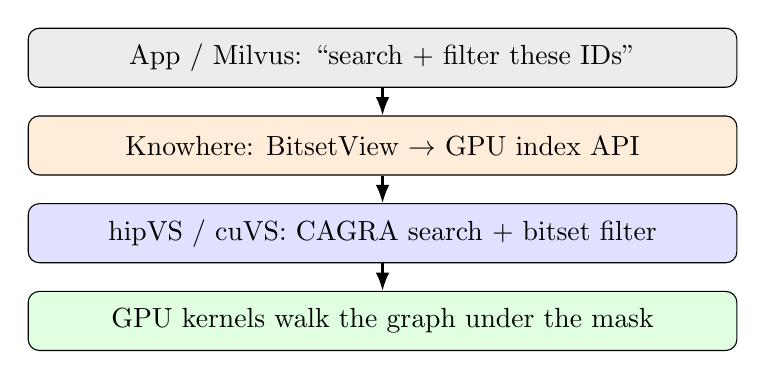
\begin{tikzpicture}[
      box/.style={draw,rounded corners,align=center,minimum width=9cm,minimum height=0.75cm},
      arr/.style={-{Latex},thick}
    ]
      \node[box,fill=gray!15] (app) {App / Milvus: ``search + filter these IDs''};
      \node[box,fill=orange!15,below=0.35cm of app] (kh) {Knowhere: BitsetView $\to$ GPU index API};
      \node[box,fill=blue!12,below=0.35cm of kh] (vs) {hipVS / cuVS: CAGRA search + bitset filter};
      \node[box,fill=green!12,below=0.35cm of vs] (gpu) {GPU kernels walk the graph under the mask};
      \draw[arr] (app) -- (kh);
      \draw[arr] (kh) -- (vs);
      \draw[arr] (vs) -- (gpu);
    \end{tikzpicture}
  \end{center}

  \vspace{0.5em}
  Our ownership proof: failure reproduces in \textbf{hipVS Python alone}\\
  (no Knowhere) $\Rightarrow$ bug is in the \textbf{library filter path}, not Milvus wiring.
\end{frame}

%======================================================================
\section{Lab}
\begin{frame}{Our lab results (plain language)}
  \footnotesize
  Host: RX 7900 XTX (\texttt{gfx1100}), hipVS Python, no Milvus.

  \vspace{0.4em}
  \begin{center}
  \begin{tabular}{@{}lcc@{}}
    \toprule
    Case & Meaning & Result \\
    \midrule
    Unfiltered & search all rows & recall@1 \textbf{1.0} (OK) \\
    Filter $\sim$40\% blocked & bitset search & recall@1 \textbf{0.0} (wrong IDs) \\
    Dense bitset (64 rows) & Catch2-like mask & \textbf{all empty} (\texttt{-1}) \\
    \bottomrule
  \end{tabular}
  \end{center}

  \vspace{0.5em}
  Also: default CAGRA graph build \texttt{ivf\_pq} often breaks on gfx1100;\\
  workaround \texttt{nn\_descent} (unfiltered then works).

  \vspace{0.4em}
  AMD Instinct blog never claims the middle rows --- only unfiltered demos.
\end{frame}

%======================================================================
\begin{frame}{Instinct blog vs consumer lab}
  \begin{center}
  \begin{tabular}{@{}p{3.6cm}p{4.2cm}p{4.2cm}@{}}
    \toprule
    & \textbf{AMD blog} & \textbf{Our lab} \\
    \midrule
    GPU class & Instinct & Radeon gfx1100 \\
    CAGRA unfiltered & Shown working & Working (\texttt{nn\_descent}) \\
    Filtered search & Not demonstrated & Broken \\
    Product filters & Out of scope & Required for Milvus \\
    \bottomrule
  \end{tabular}
  \end{center}

  \vspace{0.8em}
  \begin{block}{Correct slogan}
    ``CAGRA exists on AMD'' \textbf{yes} (Instinct demos; our unfiltered path).\\
    ``Filtered CAGRA on consumer gfx1100 is production-ready'' \textbf{not yet}.
  \end{block}
\end{frame}

%======================================================================
\begin{frame}{Glossary (cheat sheet)}
  \footnotesize
  \begin{tabular}{@{}p{3.2cm}p{10cm}@{}}
    \toprule
    Term & Meaning \\
    \midrule
    Embedding / vector & Numbers representing an item \\
    $k$ / top-$k$ & How many neighbors to return \\
    ANN & Approximate nearest neighbor search \\
    CAGRA & GPU graph ANN index (cuVS / hipVS) \\
    Unfiltered search & All indexed rows are eligible \\
    Filtered search & Only a subset of rows is eligible \\
    Bitset & Bit mask: allowed / blocked per row ID \\
    Recall@k & Fraction of true neighbors found \\
    \texttt{nn\_descent} & Graph-build algorithm (our gfx1100 workaround) \\
    \bottomrule
  \end{tabular}
\end{frame}

%======================================================================
\begin{frame}{Takeaway (send this slide alone if needed)}
  \begin{enumerate}
    \item \textbf{ANN} finds similar vectors fast using an index (CAGRA = graph on GPU).
    \item \textbf{Unfiltered} = search the whole index --- what AMD's blog shows.
    \item \textbf{Filtering} = ``skip deleted / forbidden IDs'' via a \textbf{bitset}.
    \item Milvus production needs (3); RAG demos often only need (2).
    \item On gfx1100: (2) works with \texttt{nn\_descent}; (3) is the open hipVS bug.
  \end{enumerate}

  \vspace{0.6em}
  {\footnotesize Details / repro: \texttt{docs/diy\_hipvs\_cagra\_filter\_gfx1100.md},\\
  \texttt{scripts/run\_hipvs\_cagra\_filter\_repro.sh} in \texttt{ann-harness-amd}.}
\end{frame}

\end{document}
